\documentclass{beamer}

\mode<presentation>
{
	\usetheme{default}      % or try Darmstadt, Madrid, Warsaw, ...
	\usecolortheme{default} % or try albatross, beaver, crane, ...
	\usefonttheme{default}  % or try serif, structurebold, ...
	\setbeamertemplate{navigation symbols}{}
	\setbeamertemplate{caption}[numbered]
} 

\setbeamerfont{block body}{size=\tiny}

\usepackage[english]{babel}
\usepackage[utf8x]{inputenc}
\usepackage{mathtools}

\graphicspath{ {figures/} }

\title{Machine Learning Network-Constrained Regression of Epigenetic Data}
\author{Sivo Vladimirov Daskalov}
\institute{Corpus Christi College}
\date{28 June 2017}

%Computational biology often involves working with high-dimensional data. Penalized regression methods are often used on such data, as they can perform feature selection effectively. Several approaches for network-constrained regression have been suggested in literature over the recent years. They use prior knowledge in the form of a network to exploit known relationships between predictors. An approach for cooperative parameter tuning in the context of multiple alternative methods that share common input and goals is suggested. The aim is to simultaneously tune the different regression methods iteratively, in a way that increases agreement between their coefficient estimates. We also suggest a simple approach to aggregate the coefficients produced by the various regression methods through predictor importance voting. Our method performs ordinary least squares estimation to fit the subset of predictors that have non-zero coefficients in a fraction of the underlying regression methods above a given threshold. Both tuning approaches and the various regression methods have been compared and evaluated on synthetic datasets. Gene methylation and expression data has been processed with the implemented algorithms to explore how the expression level of each gene is affected by the methylation levels of related genes.

\begin{document}
	
\begin{frame}
	\titlepage
\end{frame}

\begin{frame}{Outline}
  \tableofcontents
\end{frame}





\section{Epigenetic background}
\begin{frame}{Epigenetic background}
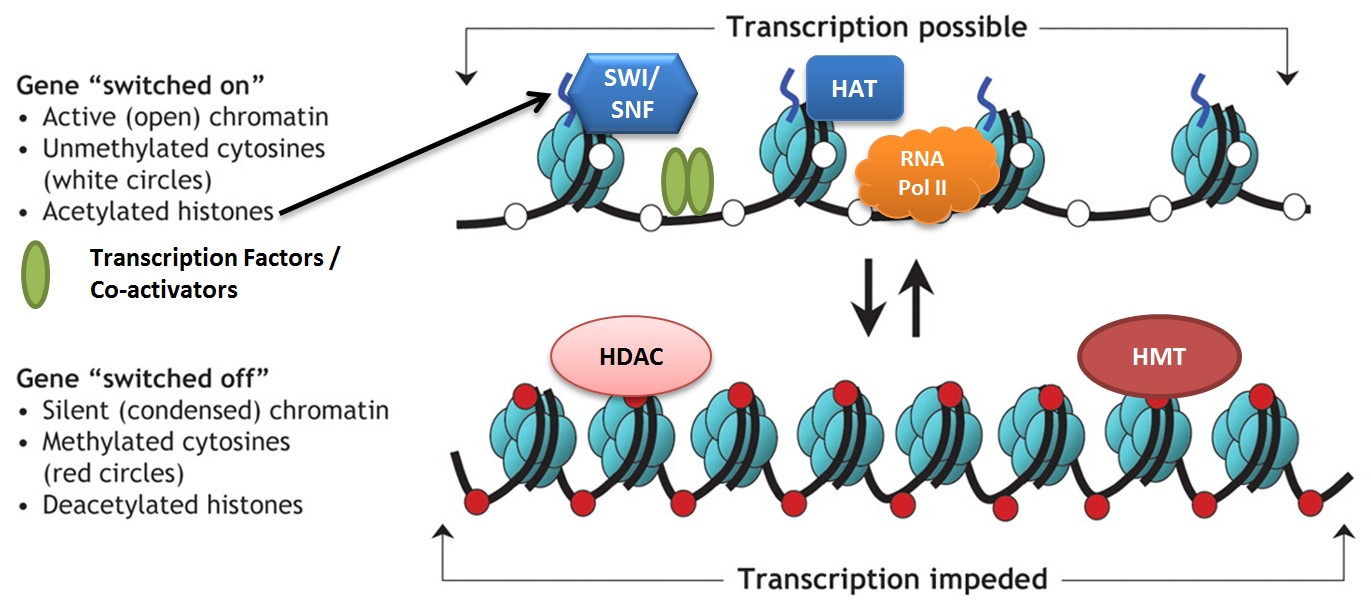
\includegraphics[width=11.5cm,height=5cm]{epigenetic_background_slide}\\
~\\~\\
\tiny{*Figure is adapted from Luong, P. Basic Principles of Genetics}
\end{frame}





\section{Project goals}
\begin{frame}{Project goals}
Question:\\
How is the expression of each gene affected by the methylation of related genes?
\\~\\~\\
Approach:\\
$\text{Linear regression}
\begin{dcases}
\text{Predictors: methylation levels for all genes}\\
\text{Target variable: expression level for gene of interest}
\end{dcases}$
\end{frame}





\section{Penalized regression methods}
\begin{frame}{Penalized regression methods}
\small
\begin{description}
	\item[Lasso] $\lambda\sum_{i=1}^{p}\left|\beta_i\right|$
	\item[Elastic Net] $\lambda_1\sum_{i=1}^{p}\left|\beta_i\right| + \lambda_2\sqrt{\sum_{i=1}^{p}\beta_i^2}$
	\item[Grace] $\lambda_1\sum_{i=1}^{p}\left|\beta_i\right| + \lambda_2\sum_{u \sim v}\left(\frac{\beta_u}{\sqrt{d_u}}-\frac{\beta_v}{\sqrt{d_v}}\right)^2w(u,v)$
	\item[aGrace] $\lambda_1\sum_{i=1}^{p}\left|\beta_i\right| + \lambda_2\sum_{u \sim v}\left(\frac{sign(\tilde{\beta}_u)\beta_u}{\sqrt{d_u}}-\frac{sign(\tilde{\beta}_v)\beta_v}{\sqrt{d_v}}\right)^2w(u,v)$
	\item[GBLasso] $\lambda\sum_{u \sim v}
	\left[\left(\frac{|\beta_u|}{\sqrt{d_u}}\right)^\gamma+
	\left(\frac{|\beta_v|}{\sqrt{d_v}}\right)^\gamma\right]^{1/\gamma}$
	\item[Linf] $\lambda\sum_{u \sim v}\max\left(\frac{|\beta_u|}{\sqrt{d_u}},\frac{|\beta_v|}{\sqrt{d_v}}\right)$
	\item[aLinf] $\lambda\sum_{u \sim v}\left|\frac{sign(\tilde{\beta}_u)\beta_u}{\sqrt{d_u}}-\frac{sign(\tilde{\beta}_v)\beta_v}{\sqrt{d_v}}\right|$
	\item[TTLP] $\lambda_1 \sum_{i=1}^{p} J_\tau|\beta_i| + \lambda_2 \sum_{u \sim v} \left|J_\tau\left(\frac{|\beta_u|}{w_u}\right)-J_\tau\left(\frac{|\beta_v|}{w_v}\right)\right|$
	\item[LTLP] $\lambda_1 \sum_{i=1}^{p}\left|\beta_i\right| + \lambda_2 \sum_{u \sim v} \left|J_\tau\left(\frac{|\beta_u|}{w_u}\right)-J_\tau\left(\frac{|\beta_v|}{w_v}\right)\right|$
\end{description}
\normalsize
\end{frame}





\section{Composite voting regression}
\begin{frame}{Composite voting regression}

{\def\arraystretch{1.5}\tabcolsep=10pt
	\begin{equation*}
	\begin{array}{l|rrrr} 
	& X_1 & X_2 & \quad\quad\quad... & X_p \\
	\hline	
	Method\ 1 & M_1(\beta_1) & M_1(\beta_2) & ... & M_1(\beta_p) \\
	Method\ 2 & M_2(\beta_1) & M_2(\beta_2) & ... & M_2(\beta_p) \\
	... & ... & ... & ... & ... \\
	Method\ k & M_k(\beta_1) & M_k(\beta_2) & ... & M_k(\beta_p)
	\end{array}
	\end{equation*}
}

\begin{equation*}
X_j = 
\begin{dcases}
important,& \text{if } \frac{\sum_{i=1}^{k}[M_i(\beta_j) \ne 0]}{k} \ge \text{fraction of votes threshold}\\
unrelated,              & \text{otherwise}
\end{dcases}
\end{equation*}

Final model obtained from OLSE on the set of important predictors
\end{frame}





\section{Orchestrated hyperparameter tuning}
\begin{frame}{Orchestrated hyperparameter tuning}
\begin{columns}[t]
	\column{.5\textwidth}
	\centering
	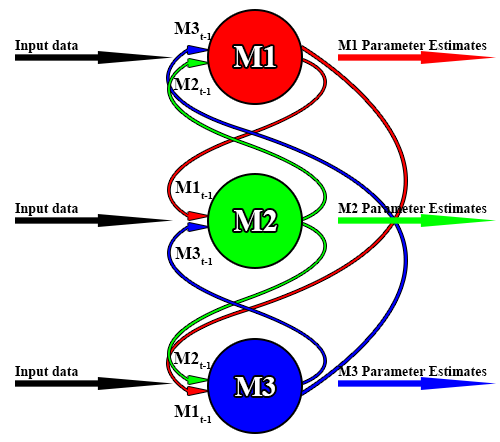
\includegraphics[width=6cm,height=5cm]{orchestrated_tuning_methodology}\\
	\column{.5\textwidth}
	\centering
	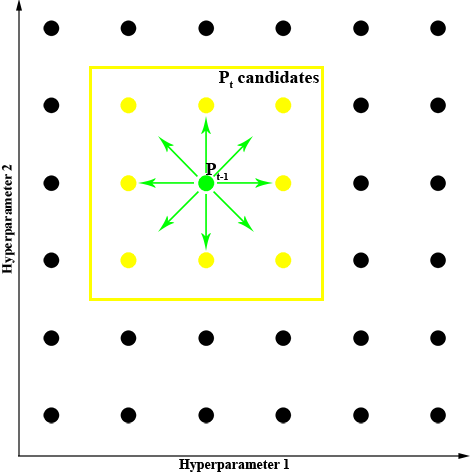
\includegraphics[width=6cm,height=5cm]{search_grid}\\
\end{columns}
\end{frame}





\section{Model evaluation}
\begin{frame}{Model evaluation}
\begin{figure}
	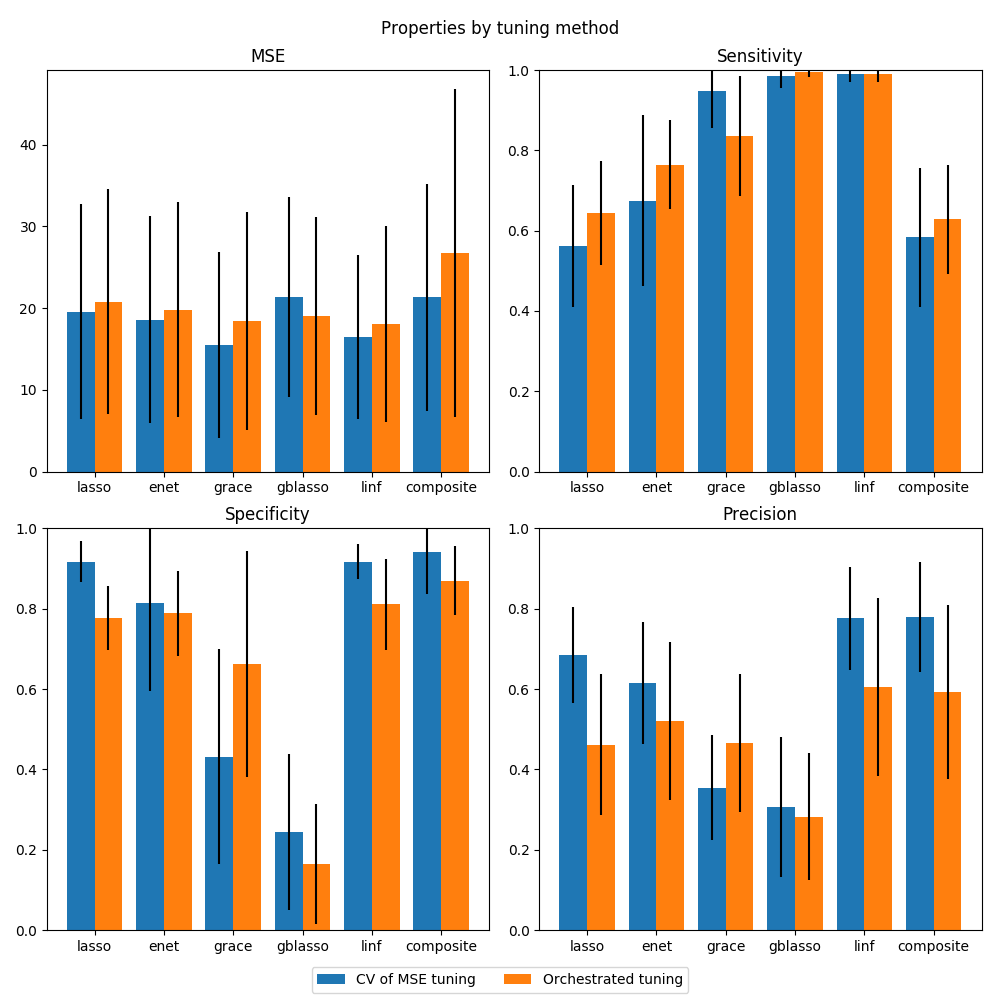
\includegraphics[width=8cm,height=8cm]{tuning_method_comparison}
\end{figure}
\end{frame}





\section{Regression method similarities}
\begin{frame}{Regression method similarities}
\begin{columns}[t]
	\column{.5\textwidth}
	\centering
	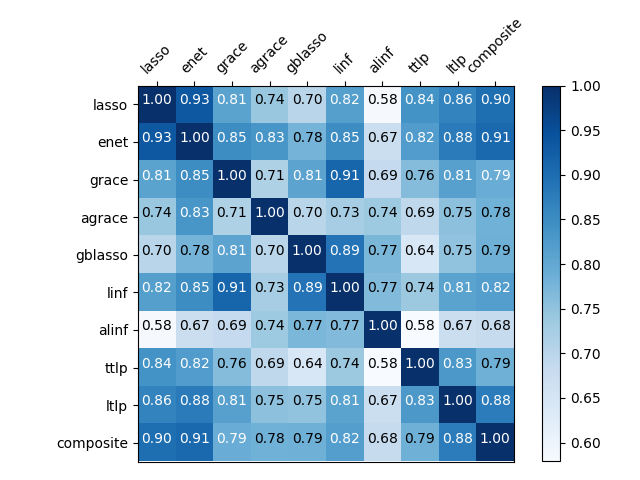
\includegraphics[width=6cm,height=5cm]{cv_mse_similarities}\\
	CV-MSE tuning
	\column{.5\textwidth}
	\centering
	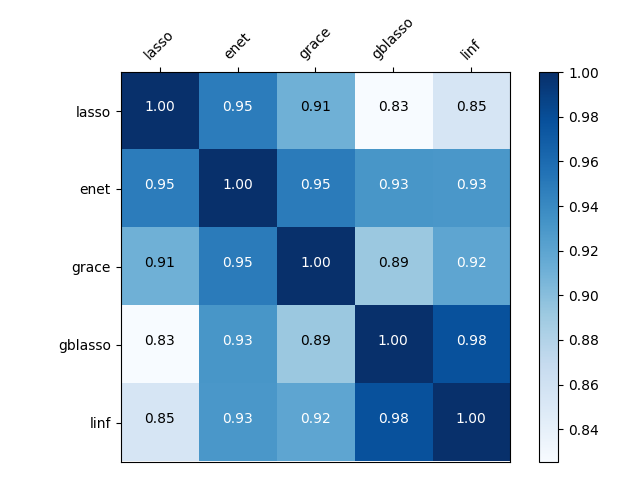
\includegraphics[width=6cm,height=5cm]{orchestrated_similarities}\\
	Orchestrated tuning
\end{columns}
\end{frame}





\section{Breast cancer dataset}
\begin{frame}{Breast cancer dataset}
\end{frame}

\end{document}